\documentclass[5p,times,twocolumn,10pt]{elsarticle}
%%%%%%%%%%%%%%%%%%%%%%%%%%%%%%%%%%%

%%%% packages and definitions (optional)
\usepackage{graphicx} % allows inclusion of graphics
\usepackage{booktabs} % nice rules (thick lines) for tables
\usepackage{microtype} % improves typography for PDF
\usepackage{xcolor}
\usepackage{amsmath}
\usepackage{amssymb}
\usepackage{caption}
\usepackage{float}
\usepackage{subcaption}
\usepackage{bm}
\usepackage{tikz}
\usepackage{verbatim}
\usetikzlibrary{arrows,shapes}
\usepackage{braket}
\usepackage[figuresright]{rotating}
\usepackage{standalone}
\usepackage[]{algorithm2e}
\usepackage{multirow}

% Define some useful commands
\newcommand{\SN}{S$_N$}
\renewcommand{\vec}[1]{\bm{#1}} %vector is bold italic
\newcommand{\vd}{\bm{\cdot}} % slightly bold vector dot
\newcommand{\grad}{\vec{\nabla}} % gradient
\newcommand{\ud}{\mathop{}\!\mathrm{d}} % upright derivative symbol
\providecommand{\e}[1]{\ensuremath{\times 10^{#1}}}
\newcommand{\oper}[1]{\mathcal{#1}}
\newcommand{\EQ}[1]{Eq.~(\ref{#1})}               %-- Eq. (refeq)
\newcommand{\EQUATION}[1]{Equation~(\ref{#1})}    %-- Equation (refeq)
\newcommand{\FIG}[1]{Fig.~\ref{#1}}               %-- Fig. refig
\newcommand{\FIGURE}[1]{\FIG{#1}}          %-- Figure refig
\newcommand{\TAB}[1]{Table~\ref{#1}}              %-- Table tablref
\newcommand{\EQS}[2]{Eqs.~(\ref{#1})--(\ref{#2})}            %-- Eqs. (refeqs)
\newcommand{\EQUATIONS}[2]{Equations~(\ref{#1})--(\ref{#2})} %-- Eqs. (refeqs)
\newcommand{\EQSTWO}[2]{Eqs.~(\ref{#1})~and~(\ref{#2})} %-- Eqs. (refeqs)
\newcommand{\EQUATIONSTWO}[2]{Equations~(\ref{#1})~and~(\ref{#2})}
%-- Eqs. (refeqs
\newcommand{\BOXEQ}[1]{\mbox{\fboxsep=.13in $$
        \framebox{#1} $$ } }    %-- box around equation
\newcommand{\SEC}[1]{Section~\ref{#1}}               %-- Eq. (refeq)
\newcommand{\REF}[1]{Ref.~\citen{#1}}               %-- Eq. (refeq)
\DeclareMathOperator*{\dotp}{{\scriptscriptstyle \stackrel{\bullet}{{}}}}

% Define how matrix and vector looks
\newcommand{\mat}[1]{\ensuremath{\bm{#1}}}
\newcommand{\mata}[1]{\ensuremath{\tilde{\bm{#1}}}}
\renewcommand{\vec}[1]{\ensuremath{\bm{#1}}}
\newcommand{\veca}[1]{\ensuremath{\tilde{\bm{#1}}}}

\begin{document}
    \begin{frontmatter}

        %% Title, authors and addresses

        \title{Effectiveness of the Discrete Generalized Multigroup Method based on truncated, POD-driven basis sets}

        \author{Richard L. Reed}
        \ead{rlreed@k-state.edu}
        \author{Jeremy A. Roberts\corref{cor1}}
        \cortext[cor1]{Phone number: 785-532-7182}
        \ead{jaroberts@k-state.edu}

        \address{
            Mechanical and Nuclear Engineering, Kansas State University, Manhattan, KS
        }

        % \ead{rlreed@k-state.edu \and jaroberts@k-state.edu}

        \begin{abstract}
            Presented is the evaluation of the discrete generalized multigroup (DGM) method using a truncated basis constructed from proper orthogonal decomposition (POD).
            The DGM method uses an orthogonal basis to collapse fine-group fluxes and cross sections to a coarse-group structure with higher order modes in each coarse-group.
            By solving the course-group equation, an approximation to the fine-group flux can be reconstructed from the course-group flux.
            This approximation is used to recollapse the cross sections, which leads to an improved approximation.
            Past development of the DGM method used the discrete Legendre polynomials (DLPs), which do not perform well under truncation for approximating the spectral shape of the flux.
            In this work, basis sets constructed using POD were used for the DGM method for several fine-group structures.
            The POD basis incorporates spectral information from small, representative problems, which are designed to capture spectral information from the full problem.
            The most effective, practical POD basis approximated the fission density with an error of less than 0.01\% relative to a reference problem using approximately 6 degrees of freedom per coarse-group for all fine-group structures.
            The reference chosen is a 1-D, repeating lattice of 10 pins of UO$_2$ fuel cells adjacent to 10 pins of 7.0\% MOX fuel pins.
            The DGM method when subject to truncation performed far better using POD basis sets than when used with the DLP basis.
        \end{abstract}

        \begin{keyword}
            Energy Expansion \sep Discrete Generalized Multigroup \sep Proper Orthogonal Decomposition
            %% keywords here, in the form: keyword \sep keyword

            %% MSC codes here, in the form: \MSC code \sep code
            %% or \MSC[2008] code \sep code (2000 is the default)

        \end{keyword}

    \end{frontmatter}

    %%%%%%%%%%%%%%%%%%%%%%%%%%%%%%%%%%%%%%%%%%%%%%%%%%%%%%%%%%%%%%%%%%%%%%%%%%%%%%%%
    \section{Introduction}

    Accurate neutronic simulations tend to require extensive computational resources for practical problems, which leads to a need for approximations.
    A common approximation is the multigroup method, which divides the continuous energy-space into a number of discrete groups.
    The cross sections are averaged over each energy range to produce the set of multigroup cross sections.
    These cross sections are then used in conjunction with the multigroup transport equation.
    Traditionally, a multi-tiered approach is used to create full-core models \cite{hebert2007review}, which condenses the energy-space while preserving reaction rates.
    However, this condensation requires an energy spectrum to weight the cross sections during the collapse.
    Since the spectrum at the core level is unknown {\it a priori}, it must be assumed, which induces errors into the core level calculations.

    The first tier begins with a continuous energy calculation in which the spatial and temporal dependence is neglected or crudely approximated.
    This calculation produces an energy spectrum that is used to compute the multigroup cross sections using hundreds or thousands of energy groups.
    Following this is typically a pin-cell calculation, where the multigroup cross sections are collapsed further to a set using on the order of tens or hundreds of energy groups which has been spatially homogenized over the pin cell.
    Next, the pin-cell multigroup cross sections are used in assembly calculations to further collapse to a coarse-group structure containing usually fewer than ten energy-groups that are homogenized over the assembly.
    The coarse-group structure and related cross sections are then used in nodal methods to simulate the whole core.

    As computational resources have increased, the desire for finer resolution at core level has also increased.
    To this end, several methods have been proposed to approximate the fine-group structure to reasonable accuracy during the full-core simulation.
    One such method is the discrete generalized multigroup method (DGM) \cite{zhu_discrete_2010, zhu_energy_2011}.
    This iterative method uses an orthogonal basis to convert a set of fine-group cross sections into a set of cross section moments mapped to a coarse-group structure.
    These coarse-group cross section moments may be used as cross sections in coarse-group calculations, which lead to coarse-group flux moments.
    The flux moments are then expanded using the basis to produce the fine-group flux spectrum.
    This fine-group flux may be used to recondense the fine-group cross sections to coarse group moments.
    This process continues iteratively until convergence, which eliminates the error from assuming the fine-group energy spectrum \cite{zhu_energy_2011, douglass_cross_2011, douglass_consistent_2012};
    however, the solution still requires full computational work due to solving the higher order moments within each coarse group.

    To reduce the required computational work, the number of degrees of freedom should be minimized for a given accuracy.
    Previous work \cite{reed2015energy} explored the use of truncated polynomials for approximating the energy variable in the response matrix method.
    The work compared the discrete Legendre polynomials (DLPs) \cite{neuman_discrete_1974} to a basis based on proper orthogonal decomposition (POD).
    The POD basis incorporates spatially-dependent spectral snapshots, which allows the low order basis vectors to closely approximate functions similar to the snapshots.
    Results showed that the POD basis performed better than the DLPs for all truncated cases.
    Similarly, positive results were found when applying such a basis to the DGM method for fixed source problems \cite{reed2017application}.
    
    The present work represents an extension to eigenvalue problems.
    These efforts are the first steps into approximations for the DGM method, which will reduce the computational and memory costs for the method.
    Previous implementations of the DGM method have used full-order, discrete basis sets, which can reproduce the fine-group solution exactly.
    This new implementation introduces truncation error into the method by reducing the number of degrees of freedom, thereby reducing the computational cost.
    Since the POD basis includes much of the functional shape in the low orders, it is expected that relatively few degreed of freedom are required for reasonable accuracy.

    This type of basis has been well studied in many fields such as image processing, and it has gained increasing attention within the nuclear community.
    The method includes the names of principle component analysis (PCA) and the Karhunen Lo\`eve transform (KLT).
    However, the method is fundamentally related to the singular value decomposition (SVD) \cite{reed2015energy}.

    \section{Background}
    \subsection{The Discrete Generalized Multigroup method}
    \label{derivation}
    What follows is a brief review of the discrete generalized multigroup (DGM) method, adapted from a previous presentation \cite{gibson_stability_2014}.
    Fundamentally, DGM is a way to represent the energy-space of a problem from within most transport approximations (e.g., discrete ordinates).
    For simplicity, we begin with the k-eigenvalue form of the 1-D, S$_n$ equations with the multigroup approximation written as
    \begin{align}
        \begin{split}
            \mu_a\frac{\partial}{\partial x}\psi_{c,a,g}
            +\Sigma^t_{c,g}\psi_{c,a,g}
            =&\sum_{l=0}^{N_l}P_l(\mu_a)\sum_{g'=1}^{N_g}\Sigma^s_{c,g\leftarrow g',l}\phi_{c,g',l}\\
            &+\frac{\chi_{c,g}}{k}\sum_{g'=1}^{N_g}\nu\Sigma^f_{c,g'}\phi_{c,g',0}\, ,
        \end{split}
        \label{eq:pn}
    \end{align}
    where
    \begin{itemize}\interlinepenalty10000\itemsep0em
        \item $\psi_{c,a,g}(x)$ is the angular flux in cell $c$ for group $g$ in the direction of angle $a$
        \item $\mu_a$ is the cosine of the angle $a$
        \item $\Sigma^t_{c,g}$ is the total cross section for group $g$ in cell $c$
        \item $\Sigma^s_{c, g\leftarrow g', l}$ is the $l$th order Legendre moment of the scattering cross section from group $g'$ to $g$ in cell $c$
        \item $k$ is the eigenvalue
        \item $\chi_{c,g}$ is the fission spectrum in cell $c$ for group $g$
        \item $\Sigma^f_{c,g'}$ is the fission cross section in cell $c$ for group $g'$
        \item $P_l(\mu_a)$ is the normalized Legendre polynomial of $l$th order evaluated at $\mu_a$
        \item $N_l$ is the order of the Legendre expansion
        \item $N_g$ is the number of energy-groups
    \end{itemize}
    and
    \begin{equation}
        \phi_{c,g,l} = \sum_{a=1}^{N_a}w_a P_l(\mu_a)\psi_{c,a,g}\, ,
    \end{equation}
    where $N_a$ is the number of discrete angles.
    $w_a$ is the weight corresponding to the discrete angle $\mu_a$ for the chosen angular quadrature scheme (e.g. Gauss Legendre).

    Now, we divide the energy-groups $g$ into a number of coarse-groups $N_G$ such that each fine-group belongs to one and only one coarse-group $G$ as
    \begin{align}
        \begin{split}
            \mu_a\frac{\partial}{\partial x}\psi_{c,a,g}
            +\Sigma^t_{c,g}\psi_{c,a,g}
            =&\sum_{l=0}^{N_l}P_l(\mu_a)\sum_{G'=1}^{N_G}\sum_{g'\in G'}\Sigma^s_{c, g\leftarrow g', l}\phi_{c, g', l}\\
            &+\frac{\chi_{c,g}}{k}\sum_{G'=1}^{N_G}\sum_{g'\in G'}\nu\Sigma^f_{c,g'}\phi_{c,g',0}\, .
        \end{split}
    \end{align}

    We introduce a set of energy-dependent, orthonormal basis vectors $P_i^G(g)$, where the subscript $i$ is the order of the basis function, and the superscript $G$ is the coarse-group for the expansion.
    Traditionally, the Legendre polynomials (both continuous and discrete) have been used as the basis vectors.
    The present work compares different basis choices against the traditional Legendre polynomials.
    More detail on the basis is provided in the next section.
    Multiplication by this basis set and summation over the coarse-group $G$ yields
    \begin{align}
        \begin{split}
            \mu_a\frac{\partial}{\partial x}\sum_{g\in G}&P_i^G(g)\psi_{c,a,g}
            +\sum_{g\in G}P_i^G(g)\Sigma^t_{c, g}\psi_{c,a,g}\\
            =&\sum_{g\in G}P_i^G(g)\sum_{l=0}^{N_l}P_l(\mu_a)\sum_{G'=1}^{N_G}\sum_{g'\in G'}
            \Sigma^s_{c, g\leftarrow g', l}\phi_{c, g', l}\\
            &+\frac{\chi_{c,g}}{k}\sum_{g\in G}P_i^G(g)\sum_{G'=1}^{N_G}\sum_{g'\in G'}\nu\Sigma^f_{c,g'}\phi_{c,g',0}\, .
            \label{eq:do-3}
        \end{split}
    \end{align}
    We define the flux moments as
    \begin{equation}
        \phi_{c,G,i,l}=\sum_{g\in G}P_i^G(g)\phi_{c,g,l}\, ,
        \label{eq:do-4a}
    \end{equation}
    and
    \begin{equation}
        \psi_{c,a,G,i}=\sum_{g\in G}P_i^G(g)\psi_{c,a,g}\, .
        \label{eq:do-4b}
    \end{equation}
    We now map the fine-group cross sections to the coarse-group structure using the definitions:
    \begin{equation}
        \Sigma^t_{c,G,0} = \frac{\sum_{g\in G}P_0^G(g)\Sigma^t_{c,g}\phi_{c,g,0}}
        {\sum_{g\in G}P_0^G(g)\phi_{c,g,0}}\, ,
        \label{eq:do-5}
    \end{equation}
    \begin{equation}
        \delta_{c,a,G,i}
        =\frac{\sum_{g\in G}P_i^G(g)\left(\Sigma^t_{c, g}-\Sigma^t_{c,G,0}\right)\psi_{c,a,g}}
        {\sum_{g\in G}P_0^G(g)\psi_{c,a,g}}\, ,
        \label{eq:do-6}
    \end{equation}
    \begin{equation}
        \Sigma^s_{c,G\leftarrow G',i,l} = \frac{\sum_{g\in G}P_i^G(g)\sum_{g'\in G'}\Sigma^s_{c, g\leftarrow g',l}\phi_{c,g',l}}
        {\sum_{g'\in G'}P_0^G(g)\phi_{c,g',l}}\, ,
        \label{eq:do-7}
    \end{equation}
    \begin{equation}
        \nu\Sigma^f_{c,G}=\frac{\sum_{g\in G}P_0^G(g)\nu\Sigma^f_{c,g}\phi_{c,g,0}}
        {\sum_{g\in G}P_0^G(g)\phi_{c,g,0}}\, ,
    \end{equation}
    \begin{equation}
        \chi_{c,G,i} = \sum_{g\in G}P_i^G(g)\chi_{c,g}\, .
        \label{eq:chi}
    \end{equation}
    Combining the definitions in \EQSTWO{eq:do-4b}{eq:do-6} yields
    \begin{equation}
        \Sigma^t_{c,G,0}\psi_{c,a,G,i}
        +\delta_{c,a,G,i}\psi_{c,a,G,0}
        =\sum_{g\in G}P_i^G(g)\Sigma^t_{c, g}\psi_{c,a,g}\, .
        \label{eq:do-8b}
    \end{equation}
    \EQUATIONS{eq:do-7}{eq:do-8b} are substituted into \EQ{eq:do-3} with \EQ{eq:do-4b} to yield
    \begin{align}
        \begin{split}
            \mu_a\frac{\partial}{\partial x}&\psi_{c,a,G,i}
            +\Sigma^t_{c,G,0}\psi_{c,a,G,i}
            +\delta_{c,a,G,i}\psi_{c,a,G,0}\\
            =&\frac{\chi_{c,G,i}}{k}\sum_{G'=1}^{N_G}\nu\Sigma^f_{c,G'}\phi_{c,G',0,0}\\
            &+\sum_{l=0}^{N_l}P_l(\mu_a)\sum_{G'=1}^{N_G}\Sigma^s_{c,G\leftarrow G',i,l}\phi_{c,G',0,l}
            \, ,
            \label{eq:DGM}
        \end{split}
    \end{align}
    which is the set of the DGM equations.
    Note that the total cross section has been split into two components $\Sigma^t_{c,G,0}$ and $\delta_{c,a,G,i}$, which represent the scalar and angular dependent components respectively.
    The term $\delta$ represents a correction for the assumption that the total cross section is isotropic, and thus only appears in the higher order terms (i.e., $\delta_{c,a,G,0}=0$).

    Also, the zeroth order solution ($i=0$) is equivalent to the standard multigroup approximation, where cross sections have been collapsed via standard procedure.
    Note that the DGM requires that $P_0^G(g)$ is the flat function, which decouples the higher order moments from eachother, i.e. so that the higher moments depend only on the zeroth moment.
    By ensuring that the zeroth moment is the flat function, all higher order basis functions will integrate to zero.
    Finally, the higher moments ($i>0$) are dependent only on the zeroth moment ($i=0$).

    \subsection{Proper Orthogonal Decomposition}
    \label{basis}
    Previous work has shown that the DLPs require many degrees of freedom to approximate the neutron flux to reasonable error, and thus do not perform well under truncation \cite{zhu_discrete_2010, zhu_discrete_2012, gibson_application_2012}.
    We seek a basis that is constructed to include physical insight.
    Such a basis would be able to approximate neutron fluxes with many fewer degrees of freedom, allowing truncation of the higher order moments without significant loss of accuracy.

    This work utilized proper orthogonal decomposition (POD) to incorporate spectral snapshots to generate an orthogonal basis.
    The central goal of POD is to approximate a discrete or continuous function $f(x)$ as a truncated expansion in an orthogonal basis whose functions yield the best possible $n$th-order approximation in terms of least-squares error for all values of $n$.
    In some applications, such as image compression, the function $f$ is predetermined, e.g., a set of pixel values.
    For other applications, such as reduced-order modeling, the function $f$ is not known.

    The method of snapshots \cite{buchan2013pod, sirovich1987turbulence} is used to generate the POD basis.
    In this work, a snapshot is an energy-dependent function that is similar to $f(x)$, i.e., the neutron flux.
    Since the neutron flux is unknown {\it a priori}, we solve a number of small, representative problems that contain features similar to our full model.
    These problems should be orders of magnitude less expensive to solve than the whole problem for practical basis generation (i.e., pin cells or assemblies used to approximate assemblies or cores respectively).
    
    The energy-dependent flux within each spatial cell of the representative (test) problem is a snapshot denoted by the vector $\vec{d}_n$.
    These vectors form the columns of the matrix $\mat{D} \in \mathbb{R}^{M\times N}$, where $M$ is the number of energy-groups, and $N$ is the number of snapshots.
    The basis is formed by first defining the matrix $\mat{B}=\mat{D}^\intercal\mat{D}$, which is semi-positive definite.
    Alternatively, the method could proceed using $\mat{D}$ instead of $\mat{B}$ as the methods are equivalent, but a semi-positive definite matrix simplifies much of the linear algebra.
    
    We perform the SVD on the matrix $\mat{B}$, which is equivalent to the eigen-decomposition for semi-positive definite matrices as
    \begin{equation}
        \mat{B}=\mat{U}_B\mat{\Sigma}_B\mat{V}_B^\intercal=\mat{Q}\mat{\Lambda}\mat{Q}^{-1}\, ,
    \end{equation}
    where $\mat{U}_B\in\mathbb{R}^{N\times N}$ and $\mat{V}_B\in\mathbb{R}^{N\times N}$ are unitary and contain the left and right singular vectors, respectively.
    The matrix $\mat{\Sigma}_B\in\mathbb{R}^{N\times N}$ is a diagonal matrix containing the singular values.
    The matrix $\mat{Q}\in\mathbb{R}^{N\times N}$ is unitary and contains the eigenvectors of $\mat{B}$ with corresponding eigenvalues contained in the diagonal matrix $\mat{\Lambda}\in\mathbb{R}^{N\times N}$.
    
    Since the matrix $\mat{B}$ is semi-positive definite, $\mat{U}_B=\mat{V}_B=\mat{Q}=\mat{V}_D$ are the right singular vectors of $\mat{D}$, and $\mat{\Lambda}_B=\mat{\Sigma}_B=\mat{\Sigma}_D^2$ are the square of the singular values of $\mat{D}$, i.e.,
    \begin{equation}
        \mat{D}^\intercal\mat{D}
        =\mat{V}_D\mat{\Sigma}_D\mat{U}_D^\intercal\mat{U}_D\mat{\Sigma}_D\mat{V}_D^\intercal
        =\mat{V}_D\mat{\Sigma}_D^2\mat{V}_D^\intercal
        =\mat{Q}\mat{\Lambda}\mat{Q}\, .
    \end{equation} 
    
    To form the POD basis, first we arrange the singular values and corresponding vectors in decreasing order, which sets the zeroth order basis as the most fundamental mode within the snapshots.
    Now, project the snapshots onto the modes as
    \begin{equation}
        \vec{p}_{j}=\mat{D}\vec{q}_j \quad \text{or}\quad \mat{P}=\mat{D}\mat{Q}\, ,
    \end{equation}
    where $\vec{q}_j$ is the $j$th column of $\mat{Q}$, and $\vec{p}_j$ is the $j$th POD basis vector.
    The resulting vectors are subsequently orthonormalized to form the basis $\mat{P}\in\mathbb{R}^{M\times N}$.
    An arbitrary length $M$ vector $\vec{f}$ may be approximately represented as
    \begin{equation}
        \vec{f}\approx\sum_{j=0}^k a_j \vec{p}_j\quad\text{where}\quad a_j=\vec{f}^\intercal \vec{p}_j\, .
    \end{equation}
    The POD basis creates the set of length $M$ basis vectors which provide the best $k$th order expansion in the least squares sense as long as the snapshots closely approximate the function $\vec{f}$.
    If $N\geq M$, then the basis $\mat{P}$ is complete and any length $M$ vector can be reproduced exactly using the first $M$ vectors of $\mat{P}$.
    
    Since the DGM method requires a flat zeroth order basis as previously mentioned, such a vector is inserted as $p_0$, and the remaining columns are shifted by one.
    The vector corresponding to the smallest eigenvalue is discarded, and the matrix $\mat{P}$ is reorthonormalized.
    This work will explore how closely the snapshots must approximate the fluxes to provide an adequate basis for the DGM method when using truncated basis sets.

    %%%%%%%%%%%%%%%%%%%%%%%%%%%%%%%%%%%%%%%%%%%%%%%%%%%%%%%%%%%%%%%%%%%%%%%%%%%%%%%%
    \section{Methods}
    \subsection{DGM Algorithm}
    To test the feasibility of using truncated basis sets within the DGM method, a 1-D discrete ordinates code was written in FORTRAN, based on a 16-angle Gauss Legendre quadrature and the diamond-difference approximation.
    This code follows the recondensation algorithm employed in previous work \cite{gibson_resonance_2013}, which is reproduced here for clarity.
    As shown in Algorithm~\ref{alg:DGM}, the method begins with fine- or ultrafine-group cross section data as well as an orthogonal basis set.
    Since the DGM method only treats the energy variable, many methods may be used to treat the spatial- and angular-space.

    Since the moments for the fission spectrum $\chi$ do not rely on the fine-group flux for collapse, as indicated in \EQ{eq:chi}, the moments are computed before beginning the recondensation loop.
    We now assume an initial shape for the fine-group flux, which will be used for initially collapsing the fluxes and cross sections into moments.
    In this work, the initial shape is set as the fine-group, fission cross sections.
    In theory, the closer the initial shape matches the solution, the fewer iterations are required for convergence.

    Within the recondensation loop, we use the fine-group flux for the current iteration and the orthogonal basis to compute the moments for the fluxes and the cross sections.
    Using these coarse-group moments, the zeroth order flux moments and k-eigenvalue are computed via a transport solver, i.e., discrete ordinates.
    The zeroth order solution is then used to solve for the higher order moments.
    As shown in \EQ{eq:DGM}, the source terms for the higher moments are dependent only on the zeroth moment, thus will converge in a single transport sweep.
    Once all moments are computed, the fine-group fluxes are reconstructed using the orthogonal basis.
    Finally, the fine-group fluxes are used to update the cross section moments within the next iteration.

    \DontPrintSemicolon
    \begin{algorithm}[htb]
        \caption{Recondensation algorithm for the DGM method}
        \KwData{cell and material properties, basis vectors}
        \KwResult{updated flux, coarse-group cross sections}
        Compute $\chi$ and $Q$ moments\;
        Guess the initial, fine-group flux\;
        \While{not converged}{
            Compute flux moments\;
            Compute cross-section moments\;
            Solve zeroth-order equations ($i=0$)\;
            Update the eigenvalue\;
            \For{all moments $i > 0$}{
                Solve $i$th-order equation\;
            }
            Reconstruct fine-group flux\;
        }
        \label{alg:DGM}
    \end{algorithm}

    Previous efforts have evaluated the stability of the DGM algorithm.
    Historically, transport sweeps through the fine-group solution were required to maintain stability, but these have been removed in favor of Krasnoselskii iteration \cite{gibson_stability_2014}.
    This iteration scheme is used to slow down a fixed point iteration (e.g., the DGM algorithm), which improves convergence.
    To briefly review, a fixed point iteration uses the solution from previous iterates to determine the initial condition for the next iteration, e.g.,
    \begin{equation}
        \vec{x}^{k+1}=\vec{F}(\vec{x}^k)\, ,
        \label{eq:picard}
    \end{equation}
    where $\vec{F}$ is an operator acting on the input $\vec{x}$ for iteration $k$.
    \EQUATION{eq:picard} depicts the simplest fixed point scheme, Picard iteration.
    This iteration scheme is stable if and only if the operator $\vec{F}$ is contractive ($||\mat{F}||\leq1$), which is not always true for the DGM algorithm.
    By introducing a parameter $\lambda\in(0,1]$, the norm of the operator can be reduced, which will improve convergence.
    This parameter is used to define Krasnoselskii iteration as
    \begin{equation}
        \vec{x}^{k+1}=(1-\lambda)\vec{x}^k + \lambda\vec{F}(\vec{x}^k)\, .
        \label{eq:Krasnoselskii}
    \end{equation}
    Notice that if $\lambda$ is set to unity, Krasnoselskii iteration reduces to Picard iteration.
    \EQUATION{eq:Krasnoselskii} is used in the DGM algorithm to compute the fine-group flux used in the next recondensation iteration.

    By adjusting the value of $\lambda$, one may select for higher computational expense in exchange for stability.
    Thus there exists an optimum value for $\lambda$, which cannot be known {\it a priori}, which produces a stable (convergent) progression with the least computational work.
    It was found that a (non-optimum) value of $\lambda=0.8$ provided stable solutions for this work.

    \subsection{Selecting Coarse group structure}
    The final necessary preparation to using the DGM method is selecting the coarse-group structure.
    Previous work \cite{gibson_stability_2014} has provided guidelines for selecting an appropriate structure that allows higher values of $\lambda$ for use in Krasnoselskii iteration.
    Those guidelines are:
    \begin{itemize}\interlinepenalty10000
        \item Limit ratio of smallest to largest $\Sigma_t$ within coarse-group
        \item Relax ratio condition for coarse-groups with small $\Sigma_t$
        \item Limit the number of fine-groups per coarse-group
        \item Force coarse-group breaks where desired
    \end{itemize}
    In this work, the ratio of smallest to largest cross section was set to 2.0.
    This ratio was ignored if the largest total cross section within the coarse group was below 1.0 cm$^{-1}$.
    Finally, a maximum of 60 fine groups were allowed within each coarse group.
    In this work, the Scale 44- and 238-group structures and the ECCO 1968-group structure were considered.
    These group structures are predefined in the continuous Monte Carlo code SERPENT \cite{leppanen2015serpent}.
    Therefore, SERPENT was used to generate a set of cross sections corresponding to each fine group structure by modeling a 2-D fuel pin with reflective conditions and homogenizing the cross sections over the material.

    The three fine group structures were collapsed to a coarse group structure using the aforementioned guidelines, which resulted in the coarse group boundaries in \TAB{tab:cg_struct}.
    The number in parenthesis in \TAB{tab:cg_struct}, i.e., the number of fine groups in a course group, is also the maximum degrees of freedom (DOF) for that coarse group.
    The order was numbered from zero, hence, a 10 DOF course group contained moments from zeroth to ninth.

    In general, the coarse-group boundaries are not evenly spaced to ensure that the total cross section is relatively flat across the coarse-group.
    Thus, the coarse-groups in the resonance region contain fewer fine-groups due to the rapid change in the cross section.
    Note that the basis is coarse-group dependent in the derivation in \SEC{derivation}.

    \begin{figure}[htb]
        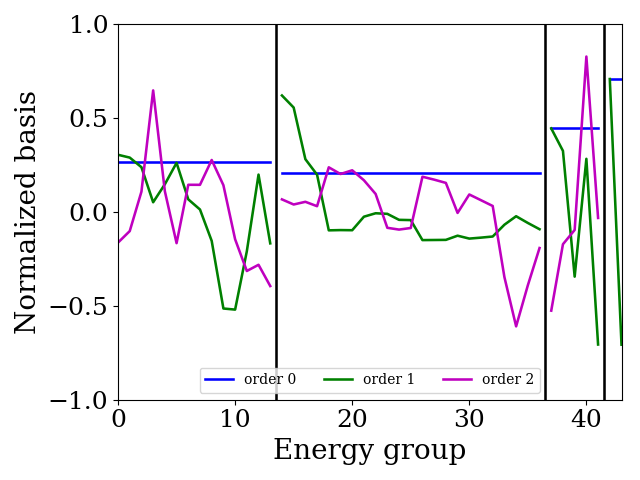
\includegraphics[scale=0.55]{figures/44_full}
        \caption{The first three vectors within each coarse group for the 44-group structure for the POD basis using ``full'' snapshots.}
        \label{fig:basis}
    \end{figure}

    The basis for each coarse group is constructed to a maximum expansion order equal to the number of DOF less one.
    For example, a coarse-group containing two DOF will contain a complete basis $\mat{B}\in\mathbb{R}^{2\times2}$.
    The POD basis as discussed in \SEC{basis} is constructed using snapshots of the flux for only the energy range corresponding to the coarse-group boundaries, i.e., the basis for each coarse-group is constructed independently as shown in \FIG{fig:basis}.
    In this work, the DGM method is explored when using a basis set truncated to order $k$, which corresponds to using only the first $k$ orders of \EQ{eq:DGM}, i.e., only the equations corresponding to $i = 0, 1, \ldots k$.

    \subsection{Infinite Medium}
    As a proof of concept, the DGM method was applied to an infinite, homogeneous UO$_2$ problem with the 44-group structure.
    In this problem, the standard DLPs are compared against a modified basis.
    The modified basis takes each DLP vector and superimposes a ``shape'' vector $s$, i.e.,
    \begin{equation}
        P_{\text{mDLP}}(g) = P_{\text{DLP}}(g)s(g)\, ,\quad g=1, 2, \ldots, N_g\, ,
    \end{equation}
    where in this case $s(g)$ is the infinite medium spectrum.
    The flat function is inserted as the zeroth vector, and the set is reorthonormalized, which creates the modified DLPs (mDLPs).
    Such a basis contains the infinite medium solution in the first two basis vectors, and should be able to capture the solution using only two degrees of freedom.
    This effect is shown in \FIG{fig:inf_med}, which presents a comparison of DLP to mDLP for solving for the maximum relative error in the fission density for the infinite medium problem.

    \begin{figure}[htb]
        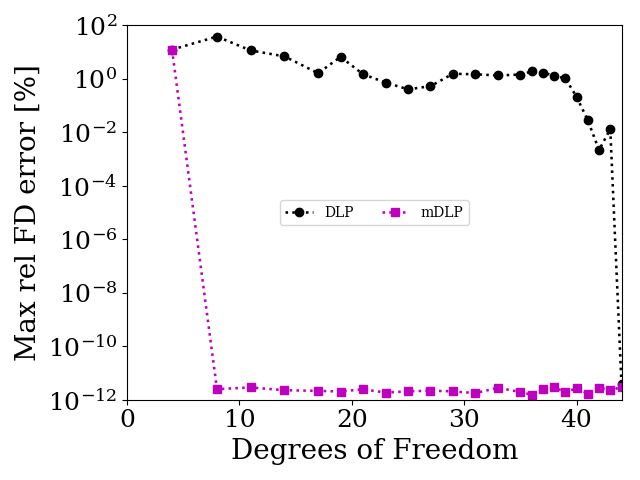
\includegraphics[scale=0.55]{figures/inf_max_fission_error_44}
        \caption{Comparison of DLP to mDLP for solving for the maximum relative error in the fission density for the infinite medium problem with the 44-group structure.}
        \label{fig:inf_med}
    \end{figure}

    Since most problems of interest are spatially dependent, a spatially-dependent basis would be required to capture the solution using only two basis vectors, which is unfeasible.
    Instead, we seek a method to use the average spectrum for a problem (or an approximation of it) as the first order vector, which should allow accurate, low-order approximations within the DGM method.

    \subsection{Test Problem}
    Shown in \FIG{fig:10-pin} is a simple 10-pin test problem adapted from previous work \cite{reed2015energy, reed2017application}.
    The problem is a 1-D, repeating lattice of UO$_2$ pins and MOX pins.
    This is modeled using five pins of UO$_2$ fuel adjacent to five pins of MOX fuel with reflective conditions on either side.
    Each pin consists of 12 fuel cells surrounded on either side by three water cells.
    Hence, the total problem contains 180 spatial cells.

    \begin{figure}[htb]
        \includestandalone[mode=buildnew, width=\columnwidth]{figures/10pin}
        \caption{Depiction of the 10-pin problem. Each fuel section (UO$_2$/MOX) used 12 mesh cells, and each moderator section (blue) used 3 mesh cells.}
        \label{fig:10-pin}
    \end{figure}

    As discussed previously, the POD basis requires a number of spectral snapshots with which to construct the orthogonal basis.
    The best snapshots would be from the full spectral shape for the 10-pin problem.
    In practical applications, these snapshots would be unavailable as the solution to the problem is required to solve the problem.
    However, the full snapshots provide insight into the best performing POD basis functions, thus are used as a comparison in this work.

    As an alternative to using the snapshots from the full problem, small representative models were created, which were used to generate sets of snapshots for basis creation.
    The first of these is an infinite lattice of UO$_2$ pins modeled as a fuel section surrounded by water with reflective boundary conditions.
    Similarly, an infinite lattice of MOX pins was created.
    These formed the UO$_2$ and MOX basis sets, respectively.
    These basis sets were expected to perform relatively poorly as snapshots from the other fuel type were missing from the basis.

    The final snapshot model considered in this work is the combined model, which is a single UO$_2$ pin modeled adjacent to a MOX pin with reflective conditions, which provides snapshots of the material junction.
    The junction snapshots were included with those from the UO$_2$ and MOX models.
    The basis created from this set of snapshots was expected to perform well as representative snapshots from all parts (infinite UO$_2$, infinite MOX, fuel junction) of the 10-pin model were included.

    \begin{figure}[htb]
        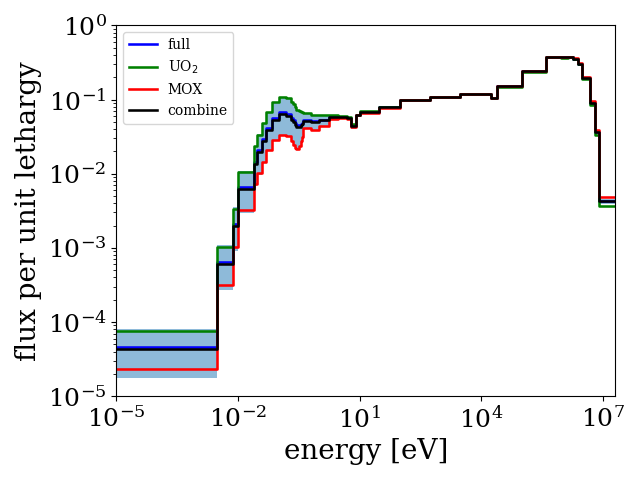
\includegraphics[scale=0.55]{figures/44_snapshots}
        \caption{Range of spatially dependent snapshots of the normalized flux per unit lethargy ($\phi(E)E$) for the 44-group, 10-pin test problem compared to the average snapshot from each snapshot model.}
        \label{fig:snapshots}
    \end{figure}

    The 10-pin problem provides 180 spatially dependent snapshots.
    The range of these snapshot spectra for the 44-group case are shown in \FIG{fig:snapshots} compared to the average spectrum from each of the snapshot models.
    Notice that the ``full'' and ``combine'' are nearly identical, which suggests a similar performance.
    The ``MOX'' and ``UO$_2$'' models, however, are significantly different.

    %%%%%%%%%%%%%%%%%%%%%%%%%%%%%%%%%%%%%%%%%%%%%%%%%%%%%%%%%%%%%%%%%%%%%%%%%%%%%%%%
    \section{Results and Analysis}

    In this section, the results from each of the three fine-group structures applied to the test problem were compared.
    The figures in this section are presented using degrees of freedom (DOF) as a metric for the amount of truncation.
    The figures show the sum of the DOF used for each coarse-group.
    For each point, we increment the number of DOF in each coarse-group by one until each coarse-group expansion is full order.
    For example, the first point for the 44-group structure is four DOF corresponding to one DOF per coarse group.
    The next points are located at eight (increasing all groups by 1), then 11 DOF (increasing the first three groups by 1 since the last group is full order).
    This reduces the space between points as coarse groups are expanded fully.

    The tests for the following figures compare the performance of truncated basis sets constructed using POD and various sets of snapshots as described in \SEC{basis}.
    The results also include a comparison to the standard discrete Legendre polynomials (DLPs).
    In \FIG{fig:maxFD}, the relative error in the total fission density is presented for the 44-, 238-, and 1968-group structures.
    The fission density is relative to a discrete ordinates solution using the same fine-group structure, the diamond difference approximation, and a 16-angle Gauss Legendre quadrature.

    \begin{figure}[!htbp]
        \centering
        \begin{subfigure}[b]{\columnwidth}
            \centering
            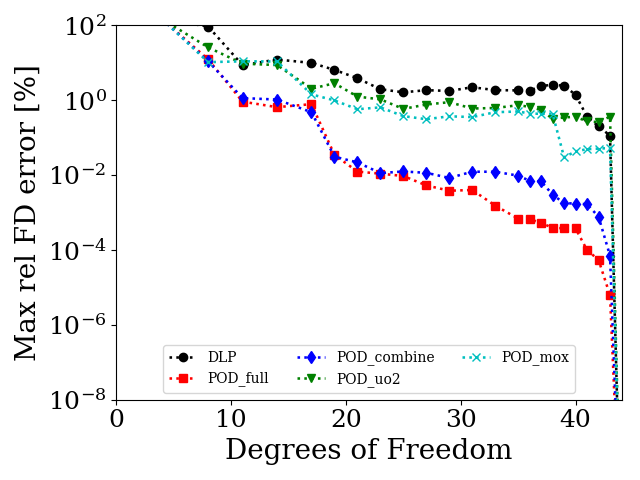
\includegraphics[scale=0.55]{figures/max_fission_error_44}
            \caption{44-group structure}
            \label{fig:maxFD44}
        \end{subfigure}
        \hfill
        \begin{subfigure}[b]{\columnwidth}
            \centering
            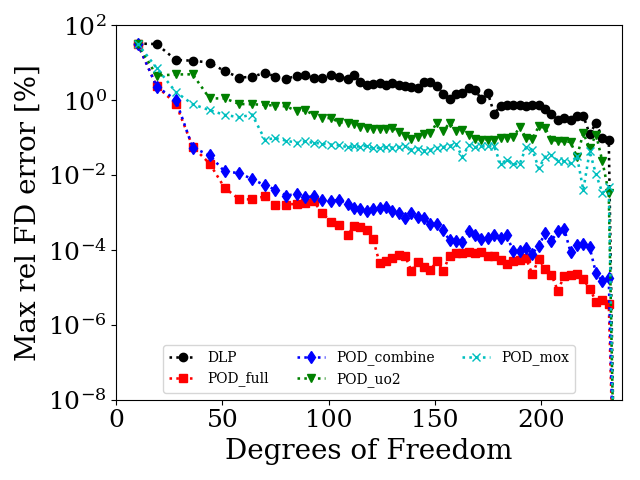
\includegraphics[scale=0.55]{figures/max_fission_error_238}
            \caption{238-group structure}
            \label{fig:maxFD238}
        \end{subfigure}
        \hfill
        \begin{subfigure}[b]{\columnwidth}
            \centering
            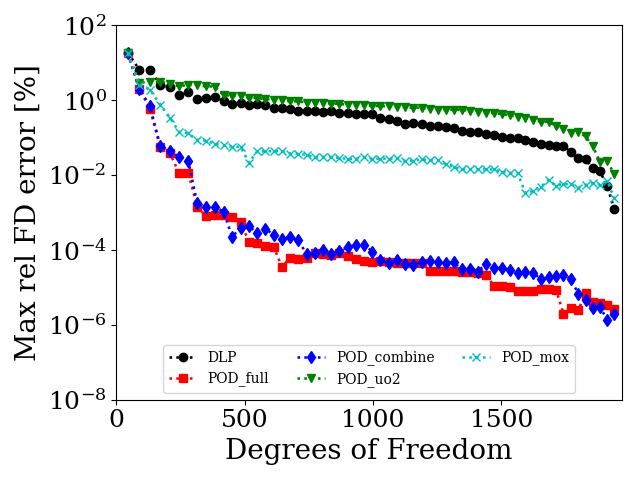
\includegraphics[scale=0.55]{figures/max_fission_error_1968}
            \caption{1968-group structure}
            \label{fig:maxFD1968}
        \end{subfigure}
        \caption{Maximum error in total fission density (FD) relative to a discrete ordinates solution as a function of DOF for various truncated basis sets}
        \label{fig:maxFD}
    \end{figure}

    In general, the POD basis performs better than the DLPs because the spectral shape of the flux requires a high-order expansion in the DLPs to be effective.
    All of the basis types converge within double precision tolerance to the reference solution at full order.
    The POD basis constructed using snapshots of the full problem is the best, but this basis required the solution {\it a priori}, thus is not practical.

    The combined basis performs nearly as well reaching approximately 0.01\% error using only 6 DOF per coarse group.
    The UO$_2$ and MOX basis sets do not perform well because the spectral information is missing from other half of the fuel types.
    The same general trends are present in each of the group structures, and approximately the same number of DOF per coarse-group are required to achieve a given accuracy.

    \begin{figure}[!htbp]
        \centering
        \begin{subfigure}[b]{\columnwidth}
            \centering
            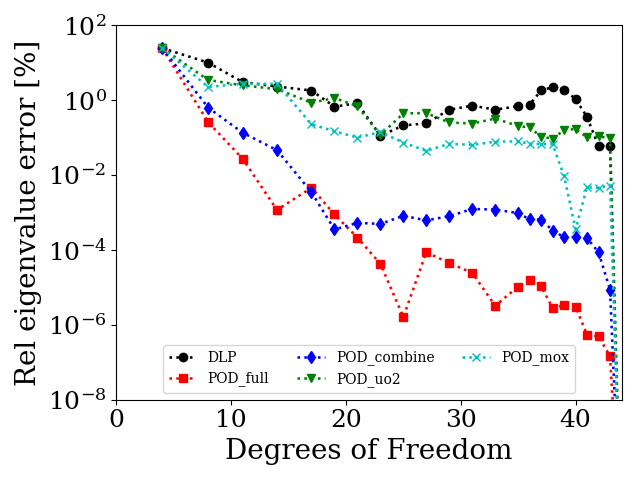
\includegraphics[scale=0.55]{figures/k_error_44}
            \caption{44-group structure}
            \label{fig:k44}
        \end{subfigure}
        \hfill
        \begin{subfigure}[b]{\columnwidth}
            \centering
            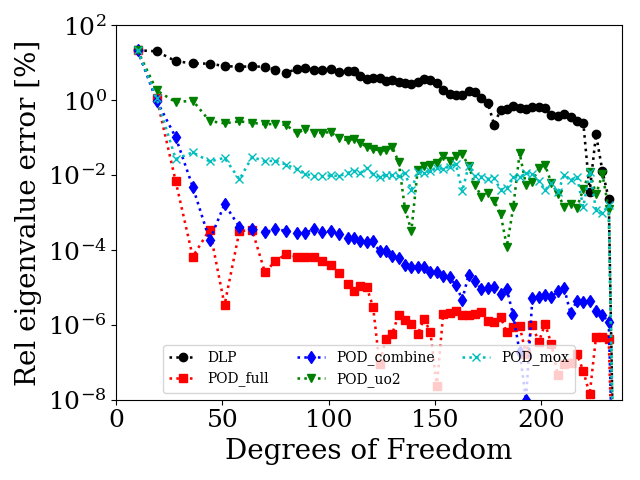
\includegraphics[scale=0.55]{figures/k_error_238}
            \caption{238-group structure}
            \label{fig:k238}
        \end{subfigure}
        \hfill
        \begin{subfigure}[b]{\columnwidth}
            \centering
            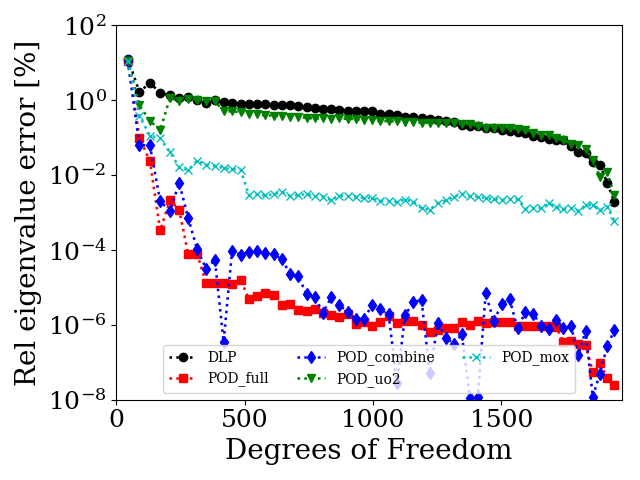
\includegraphics[scale=0.55]{figures/k_error_1968}
            \caption{1968-group structure}
            \label{fig:k1968}
        \end{subfigure}
        \caption{Error in eigenvalue relative to a discrete ordinates solution as a function of DOF for various truncated basis sets}
        \label{fig:k}
    \end{figure}

    The error in the eigenvalue for the test problem is presented in \FIG{fig:k}.
    The relative performance of the basis sets is similar to the previous results.
    Also, note that the magnitude of the error is smaller for the eigenvalue as compared to the fission density.

    %%%%%%%%%%%%%%%%%%%%%%%%%%%%%%%%%%%%%%%%%%%%%%%%%%%%%%%%%%%%%%%%%%%%%%%%%%%%%%%%
    \section{Conclusions}
    The DGM method has been suggested as a way to use computational work on the order of a coarse-group solution to accurately approximate a fine-group solution.
    In this work we explored an improvement to the DGM method, which allows the computational requirements to be further reduced.

    Previous work has used the discrete Legendre polynomials (DLP) to collapse the fluxes and cross sections within the DGM method.
    However, this work has used a basis constructed to include spectral information (i.e., group-dependent flux in a given cell) using proper orthogonal decomposition (POD) and the method of snapshots.
    Alone, such a basis will provide no improvement as compared to DLP because both basis sets are complete.
    However, this work also explored using a truncated basis in conjunction with the DGM method.
    The POD basis is constructed such that the spectral information is concentrated in the low orders, which means the basis can be used for accurate reconstruction using few degrees of freedom (DOF).

    This work has shown that the DGM method can successfully be used with a truncated basis set for a simple test problem.
    We find that the POD basis constructed using spectral information from all materials will perform better than a basis lacking a fuel type for example.
    The best POD basis is constructed using snapshots of the true solution, but these are impractical to use as the solution is required to approximate the solution.
    However, by combining snapshots of representative problems, a basis was constructed that performed similarly to the best basis for the low order approximations.

    This work shows that the POD basis performs comparably with several group structures, and requires approximately the same number of DOF per coarse-group for a chosen accuracy.
    In fact, approximately 0.01\% relative error in the fission density can be achieved with around six DOF per coarse-group.
    Further, using a higher number of groups for the fine-group structure improves the relative performance of DGM compared to discrete ordinates.
    Note that the DGM method is a way to treat the energy variable, and is independent of the chosen spatial or angular solver.

    %%%%%%%%%%%%%%%%%%%%%%%%%%%%%%%%%%%%%%%%%%%%%%%%%%%%%%%%%%%%%%%%%%%%%%%%%%%%%%%%
    \section{Acknowledgments}
    The work of the first author was supported by the Kansas State University Nuclear Research Fellowship Program, generously sponsored by the U.S. Nuclear Regulatory Commission (Grant NRC-HQ-84-14-G-0033).

    %%%%%%%%%%%%%%%%%%%%%%%%%%%%%%%%%%%%%%%%%%%%%%%%%%%%%%%%%%%%%%%%%%%%%%%%%%%%%%%%
    \section{References}
    \bibliographystyle{elsarticle-num}
    \bibliography{references}

    \appendix
    \onecolumn
    \section{Coarse Group Bounds}
    The three fine group structures used in this work are presented in \TAB{tab:cg_struct}, where the energy groups are in decreasing energy order.
    The number in parenthesis in \TAB{tab:cg_struct}, i.e., the number of fine groups in a course group, is also the maximum degrees of freedom (DOF) for that coarse group.
    \begin{table*}[htb]
        \centering
        \caption{Fine-group to coarse-group mapping.  The number in parenthesis is the number of fine-groups within the coarse-group.}
        \begin{tabular}{c|cc|cc|cccccccc}\toprule
            Group & \multicolumn{2}{|c|}{44-group} & \multicolumn{2}{|c|}{238-group}
            & \multicolumn{8}{c}{1968-group}
            \\ \midrule
            1 &1-14 &(14)&1-14   &(14)&1-10   &(10)&671-730  &(60)&1391-1392&(2) &1654-1658&(5)\\
            2 &15-37&(23)&15-74  &(60)&11-70  &(60)&731-790  &(60)&1393-1447&(55)&1659-1665&(7)\\
            3 &38-42&(5) &75-134 &(60)&71-130 &(60)&791-850  &(60)&1448-1450&(3) &1666-1725&(60)\\
            4 &43-44&(2) &135-137&(3) &131-190&(60)&851-910  &(60)&1451-1464&(14)&1726-1785&(60)\\
            5 &     &    &138-156&(19)&191-250&(60)&911-970  &(60)&1465-1466&(2) &1786-1796&(11)\\
            6 &     &    &157-216&(60)&251-310&(60)&971-1030 &(60)&1467-1517&(51)&1797-1835&(39)\\
            7 &     &    &217-225&(9) &311-370&(60)&1031-1090&(60)&1518-1519&(2) &1836-1895&(60)\\
            8 &     &    &226-232&(7) &371-430&(60)&1091-1150&(60)&1520-1526&(7) &1896-1955&(60)\\
            9 &     &    &233-237&(5) &431-490&(60)&1151-1210&(60)&1527-1586&(60)&1956-1964&(9)\\
            10&     &    &238    &(1) &491-550&(60)&1211-1270&(60)&1587-1590&(4) &1965-1968&(4)\\
            11&     &    &       &    &551-610&(60)&1271-1330&(60)&1591-1593&(3) &         &\\
            12&     &    &       &    &611-670&(60)&1331-1390&(60)&1594-1653&(60)&         &\\
            \bottomrule
        \end{tabular}

        \label{tab:cg_struct}
    \end{table*}

\end{document}
